% Options for packages loaded elsewhere
\PassOptionsToPackage{unicode}{hyperref}
\PassOptionsToPackage{hyphens}{url}
\documentclass{beamer}
\usepackage{graphicx}
\usepackage{amsmath}
\usepackage{booktabs}
\usepackage{xcolor}
\usepackage{bookmark}

% Penn colors
\definecolor{pennred}{HTML}{990000}
\definecolor{pennblue}{HTML}{011f5b}

% Beamer theme settings
\usetheme{Madrid}
\setbeamercolor{structure}{fg=pennred}
\setbeamercolor{frametitle}{bg=pennblue, fg=white}
\setbeamercolor{title}{fg=white}
\setbeamercolor{item}{fg=pennred}

\title[Beyond Expected Goals]{Beyond Expected Goals: A Probabilistic Framework for Shot Occurrences in Soccer}
\author[Pipping, Feng, and Sabin]{Jonathan Pipping, Tianshu Feng, and Paul Sabin}
\date{August 7, 2025}
\institute[UPenn]{University of Pennsylvania}

\begin{document}

\frame{\titlepage}

% What Are Expected Goals (xG)?
\begin{frame}{What Are Expected Goals (xG)?}
\begin{itemize}
\item Expected Goals (xG) is a metric that estimates the probability that a shot is scored
\item Depends on factors like distance from goal, angle to goal, shot type, and player positions
\item Estimated by XGBoost models trained on historical shot data
\item Often used to measure the quality of a chance
\item Aggregated over a match or season to measure team performance
\end{itemize}
\end{frame}

% Limitations of xG
\begin{frame}{Limitations of xG}
\begin{itemize}
\item Models are only trained on \textbf{observed} shots, inducing significant selection bias
\item Skilled attackers who take more shots are over-represented
\item Threatening attacks with no recorded shots are omitted
\item Aggregating xG across a match double-counts rebound chances
\end{itemize}
\end{frame}

% Visual Examples
\begin{frame}{Example 1: No Shot Recorded}

\end{frame}

\begin{frame}{Example 2: Multiple Shots Taken}

\end{frame}

% Our Target Metric: xG+
\begin{frame}{Our Target Metric: xG+}
\begin{itemize}
\item A more complete picture of goal expectancy
  \begin{itemize}
  \item Accounts for high-threat attacks with no shots
  \item Avoids double-counting rebounded chances
  \end{itemize}
\item At each frame $t$, let xG+ be the probability of a goal:
\begin{align*}
\text{xG+}_t &= \mathbb{P}_t(\text{goal scored}) \\
&= \mathbb{P}_t(\text{goal scored} \mid \text{shot taken})\cdot\mathbb{P}_t(\text{shot taken}) \\
&= \text{xG}_t\cdot\text{xShot}_t
\end{align*}
\item Then define xG+ over a possession with $n$ frames:
$$\text{xG+}_\text{poss} = 1 - \prod \left(1 - \mathbb{P}_t\left(\text{goal scored}\right)\right)$$
\item Estimating this value requires fitting two models: xG and xShot
\end{itemize}
\end{frame}

% Data Overview
\begin{frame}{Data Overview}
\begin{itemize}
\item \textbf{Source:} Pro Football Focus (PFF) FC video tracking and event data from the 2022-2025 English Premier League
\item \textbf{Key Features:}
  \begin{itemize}
  \item Player positions (x, y) at 30 frames per second
  \item Ball position (x, y, z) at 30 frames per second
  \item Shot events and outcomes
  \item Team possession indicators
  \item Player and team identifiers
  \end{itemize}
\end{itemize}
\end{frame}

% Data Cleaning
\begin{frame}{Data Cleaning}
\begin{itemize}
\item \textbf{Filtering:} Keep frames where the ball is in play and a team has clear possession
\item \textbf{Smooth Ball Tracking:} Linearly interpolate ball positions to fill in missing frames
\item \textbf{Define Attacking Sequences:}
  \begin{itemize}
  \item Start: team gains possession in their attacking third
  \item End: defending team regains possession or ball exits attacking third
  \end{itemize}
\item \textbf{Field Standardization:} Flip right-to-left attacks $180^{\circ}$ to make all attacks go left-to-right
\end{itemize}
\end{frame}

% Feature Engineering
\begin{frame}{Feature Engineering}
\begin{itemize}
\item \textbf{Ball Features:}
  \begin{itemize}
  \item Distance from goal ($r_{ball}$)
  \item Angle to goal ($\theta_{ball}$)
  \item Ball height ($z_{ball}$)
  \item Ball speed ($v_{ball}$)
  \end{itemize}
\item \textbf{Player Features:}
  \begin{itemize}
  \item Position of 5 closest offensive teammates relative to the ball ($r_{off}, \theta_{off}$)
  \item Position of 5 closest non-GK defenders relative to the ball ($r_{def}, \theta_{def}$)
  \item Position of goalkeeper relative to the goal ($r_{gk}, \theta_{gk}$)
  \end{itemize}
\item \textbf{Goal Openness:}
  \begin{itemize}
    \item Model defenders as circles with diameter 0.75m
    \item Draw tangent lines from the ball to defenders and find where they meet the goal line
    \item Call the percentage of the goal that's unobstructed \texttt{openGoal}
  \end{itemize}
\end{itemize}
\end{frame}

% Modeling xShot
\begin{frame}{Modeling}
\begin{itemize}
  \item \textbf{Training Data:} All data from the 2022-2025 Premier League seasons
  \item \textbf{Features:} Ball features, player features, and goal openness
  \item \textbf{xG}: 5-fold cross-validated XGBoost model estimating the probability that a shot is scored
  \item \textbf{xShot}: 5-fold cross-validated XGBoost model estimating the probability that a shot occurs \emph{in the next second}

  \item \textbf{Evaluation Metric:} Log loss
\end{itemize}
\end{frame}

% Results
\begin{frame}{Results}
\begin{columns}[c]
  \column{0.4\textwidth}
  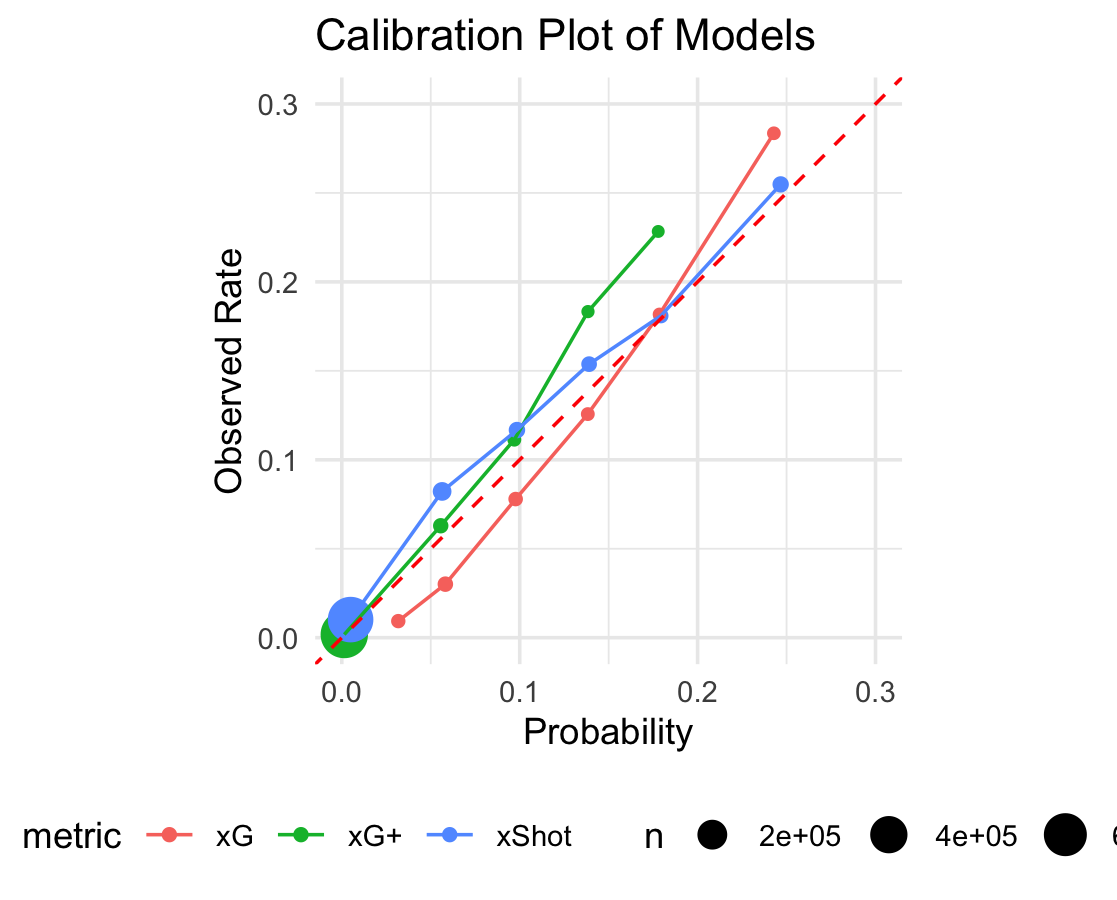
\includegraphics[width=\linewidth]{figures/calibration_1.png}
  
  \column{0.4\textwidth}
  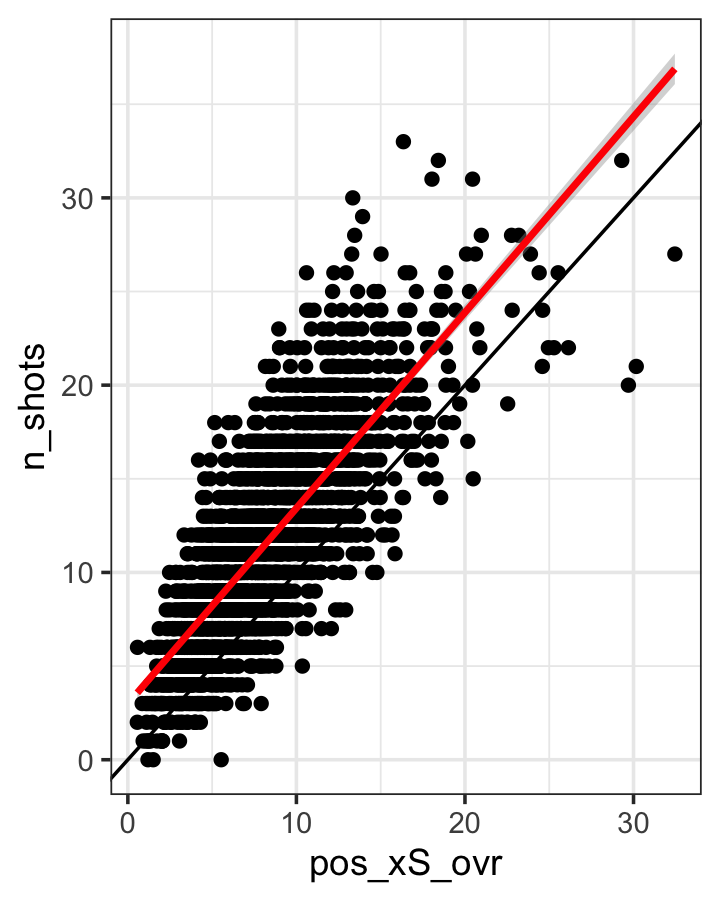
\includegraphics[width=\linewidth]{figures/calibration_2.png}
\end{columns}
\end{frame}

% Cross-Validation Study
\begin{frame}{Cross-Validation Study}
\begin{itemize}
\item \textbf{Objective}: Evaluate xG+ performance using cross-validated Poisson models
\item \textbf{Dataset}: 3 seasons of match data (114 folds total)
\item \textbf{Method}: Train on all matchdays except one, predict goals on held-out data
\item \textbf{Goal}: Determine how well adjusted xG+ explains actual goals scored
\end{itemize}
\end{frame}

% Cross-Validation Setup
\begin{frame}{Cross-Validation Setup}
\begin{itemize}
\item Each matchday treated as a fold: $38 \text{ matchdays} \times 3 = 114$ folds
\item For each fold:
  \begin{itemize}
  \item Train on all matchdays except one to acquire adjusted metrics
  \item Poisson regression on team goals using training data
  \item Predict goals scored on held-out matchday test data
  \end{itemize}
\end{itemize}
\end{frame}

% Metrics and Aggregation Methods
\begin{frame}{Metrics and Aggregation Methods}
\textbf{Metrics:}
\begin{itemize}
\item \textbf{xS}: Probability a player takes a shot in the next second
\item \textbf{xG}: Probability of a goal (given a shot)
\item \textbf{xG+}: xS $\times$ xG, probability of scoring in the next second
\end{itemize}

\textbf{Aggregation Methods:}
\begin{enumerate}
\item \textbf{Max-per-possession}: Take maximum 1-second prediction in each possession
\item \textbf{At-least-one-per-possession}: $1 - \prod (1 - p)$ across possession
\item \textbf{Sum-of-shots}: Traditional xG summed over actual shots
\end{enumerate}
\end{frame}

% Mixed Effects Modeling
\begin{frame}{Mixed Effects Modeling}
\textbf{Fitted on training data for each fold:}
$$\texttt{metric} \sim (1|\texttt{season}) + (1|\texttt{season:team}) + (1|\texttt{season:opp}) + \texttt{home}$$

\textbf{Extracted effects:}
\begin{itemize}
\item Team attack (per season)
\item Opponent defense (per season)
\item Season effect
\item Home field advantage
\end{itemize}
\end{frame}

% Secondary Poisson Model
\begin{frame}{Secondary Poisson Model}
\textbf{Train Poisson regression on adjusted metrics:}
$$\texttt{goals} \sim \texttt{home} + \texttt{season} + \texttt{team\_off} + \texttt{opp\_def}$$

\textbf{Purpose}: Assess predictive utility of each adjusted metric on actual goals
\end{frame}

% Cross-Validation Results
\begin{frame}{Cross-Validation Results}
\begin{table}[!h]
\centering
\caption{Mean Squared Error (MSE) by Metric and Aggregation Method}
\begin{tabular}[t]{lrrr}
\toprule
Aggregation Method & xG+ & xS & xG\\
\midrule
At-least-one-per-possession & 2.84 & 2.90 & 2.94\\
Max-per-possession & 2.84 & 2.87 & 2.91\\
Sum-of-shots &  &  & 2.90\\
\bottomrule
\end{tabular}
\end{table}
\end{frame}

\begin{frame}{Cross-Validation Results}
\begin{table}[!h]
\centering
\caption{Mean Absolute Error (MAE) by Metric and Aggregation Method}
\begin{tabular}[t]{lrrr}
\toprule
Aggregation Method & xG+ & xS & xG\\
\midrule
At-least-one-per-possession & 1.86 & 1.87 & 1.89\\
Max-per-possession & 1.86 & 1.86 & 1.89\\
Sum-of-shots &  &  & 1.87\\
\bottomrule
\end{tabular}
\end{table}
\end{frame}

% Conclusions
\begin{frame}{Conclusions}
\begin{itemize}
\item \textbf{xG+ performs best}: Lowest MSE and MAE across all aggregation methods
\item \textbf{At-least-one-per-possession} aggregation method shows strongest performance
\item \textbf{Future work}: Compare to actual shot-based xG, consider time-weighted xS
\item \textbf{Questions and discussion}
\end{itemize}
\end{frame}

% Acknowledgements
\begin{frame}{Acknowledgements}
\begin{itemize}
\item Special thanks to our data providers at PFF FC and the English Premier League.
\item All work supported by the Wharton Sports Analytics \& Business Initiative (WSABI) Summer Research Lab.
\end{itemize}
\end{frame}

\end{document}